\let\negmedspace\undefined
\let\negthickspace\undefined
\documentclass[journal,12pt,twocolumn]{IEEEtran}

 \usepackage{gensymb}

 \usepackage{polynom}

\usepackage{amssymb}

\usepackage[cmex10]{amsmath}
\usepackage{amsthm}
\usepackage{graphicx}

 \usepackage{stfloats}

 \usepackage{bm}
\usepackage{longtable}

\usepackage{enumitem}
 

\DeclareMathOperator*{\Res}{Res}
\DeclareMathOperator*{\equals}{=}


\begin{document}

\bibliographystyle{IEEEtran}


\providecommand{\pr}[1]{\ensuremath{\Pr\left(#1\right)}}
\providecommand{\qfunc}[1]{\ensuremath{Q\left(#1\right)}}
\providecommand{\sbrak}[1]{\ensuremath{{}\left[#1\right]}}
\providecommand{\lsbrak}[1]{\ensuremath{{}\left[#1\right.}}
\providecommand{\rsbrak}[1]{\ensuremath{{}\left.#1\right]}}
\providecommand{\brak}[1]{\ensuremath{\left(#1\right)}}
\providecommand{\lbrak}[1]{\ensuremath{\left(#1\right.}}
\providecommand{\rbrak}[1]{\ensuremath{\left.#1\right)}}
\providecommand{\cbrak}[1]{\ensuremath{\left\{#1\right\}}}
\providecommand{\lcbrak}[1]{\ensuremath{\left\{#1\right.}}
\providecommand{\rcbrak}[1]{\ensuremath{\left.#1\right\}}}
\theoremstyle{remark}
\newtheorem{rem}{Remark}
\newcommand{\sgn}{\mathop{\mathrm{sgn}}}

\providecommand{\system}{\overset{\mathcal{H}}{ \longleftrightarrow}}
\newcommand{\question}{\noindent \textbf{Question: }}	
\newcommand{\solution}{\noindent \textbf{Solution: }}

\providecommand{\dec}[2]{\ensuremath{\overset{#1}{\underset{#2}{\gtrless}}}}

\let\vec\mathbf

\newcommand{\myvec}[1]{\ensuremath{\begin{pmatrix}#1\end{pmatrix}}}
\newcommand{\mydet}[1]{\ensuremath{\begin{vmatrix}#1\end{vmatrix}}}

\vspace{3cm}
\title{I.C.S.E 10, 2018}

\author{ Burra Vishal Mathews\\CS21BTECH11010}
	


\maketitle
\question : 3(a) : 
 If $(x+2)$ and $(x+3)$ are factors of $x^3+ax+b$, find the values of $'a'$ and $'b'$.\\


\solution
    According to the question :

    $x+2$ and $x+3$ are factors of $x^3+ax+b$.\\
    Then, -2 and -3 are solutions of the equation \\
    \begin{equation}
    \label{maineq}
        x^3+ax+b=0 
    \end{equation}
    On substituting $x=-2$  int the equation \eqref{maineq}
        $$\implies \brak{-2}^3+a\brak{-2}+b=0$$ 

    \begin{equation}
    \label{eq1}
        \implies 2a-b=-8
    \end{equation}

    On substituting $x=-3$ in the equation \eqref{maineq}$$\implies \brak{-3}^3+a\brak{-3}+b=0$$
    \begin{equation}
    \label{eq2}
        \implies 3a-b=-27
    \end{equation}
    
    The system of equations ,
    $$2a-b=-8$$
    $$3a-b=-27$$
    can be re-written in matrix form as :
    $$\myvec{2&-1\\3&-1}\myvec{a\\b}\equals\myvec{-8\\-27}$$
    Let, $i$th row is a matrix be represented as $R_i$ .\\
    The system of equations ,
    $$a_1x+b_1y=c_1$$
    $$a_2x+b_2y=c_2$$
    if represented as :
    \myvec{\begin{array}{c c|c}
        a_1 & b_1 &c_1 \\
        a_2 & b_2& c_2\\ 
    \end{array}}\\
    Solution of such system of equations is $x_1$ $\And$ $y_1$ where matrix is reduced using row transformation to ;\\
    \begin{center}
       \myvec{\begin{array}{cc|c}
        1 & 0&x_1 \\
        0& 1& y_1\\ 
        \end{array}}\\
    \end{center}
    For given system of equations,\\
    
    \begin{center}
        \myvec{\begin{array}{cc|c}
            2& -1&-8 \\
            3& -1&-27\\
        \end{array}}\\
    \end{center}
    \textbf{Transformation 1 :} $R_1 \rightarrow R_2-R_1$\\
    
    $\implies$
    \myvec{\begin{array}{cc|c}
        1& 0&-19 \\
        3& -1&-27\\
    \end{array}}\\
    \textbf{Transformation 2 :} $R_2\rightarrow 3R_1-R_2$\\
    
    $\implies$
    \myvec{\begin{array}{cc|c}
        1& 0&-19 \\
        0& 1&-30
    \end{array}}
    
    

    $ \therefore $ The value of $a = -19$ and value of $b = -30$.\\
    
    Using values of $a$ and $b$, equation \eqref{maineq} can be re-written as :
    \begin{equation}
    \label{Peq}
        x^3-19x-30=0
    \end{equation}
    This can be verified by plotting the graph of the equation
    \begin{equation}
    \label{grapheq}
        y=x^3-19x-30
    \end{equation}
    
\begin{figure}[h]
    \includegraphics[width=0.9\columnwidth]{figs/graph.png}
    \caption{Graph of equation. \eqref{grapheq} intersects X-axis at $x=-3$ $\And$ $x=-2$ }
    \label{graph}

\end{figure}
\newpage
Output of python code which checks if both 'a' and 'b' are solutions of the equations \eqref{eq1} and \eqref{eq2}
\begin{figure}[h]
    \centering
    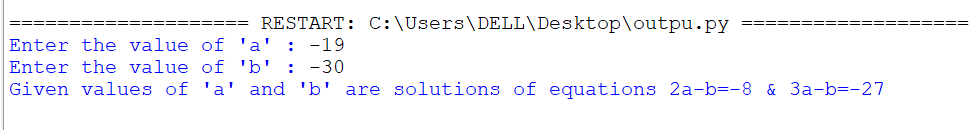
\includegraphics[width=\columnwidth]{figs/output.png}
    \caption{Output of given code.}
    \label{op}
\end{figure}

\end{document}